\documentclass[french,a4paper,10pt]{article}
% pdflatex compte_rendu.tex -output-directory=out && mv out/compte_rendu.pdf ./

\usepackage[a4paper,hmargin=30mm,vmargin=30mm]{geometry}
\usepackage[T1]{fontenc} % font type
\usepackage[french]{babel} % language
\usepackage{lmodern} % font type
\usepackage[shortlabels]{enumitem}
\usepackage{hyperref}
\usepackage{graphicx}
\usepackage{sectsty}
%\setlength{\parindent}{0pt}



\title{Compte Rendu TP2\\Opérations morphologies sur des images}
\author{Ivan Lejeune}
\date{\today}


\begin{document}
	\maketitle

	% make table of contents
	\tableofcontents

	\newpage
	\section{Seuillage d'une image et erosion de l'image binaire}\label{sec:1}

	\subsection{Choix de l'image}\label{subsec:1.1}

	On commence par choisir une image au format \emph{pgm}, dans notre cas, l'image \texttt{08.pgm}.
	On réduit ensuite la taille de l'image pour faciliter le traitement, on choisit une taille de 256x256 pixels.
	Cela donne alors :
	% insert original image and resized image
	\begin{figure}[!htb]
		\begin{minipage}{0.48\textwidth}
			\centering
			\fbox{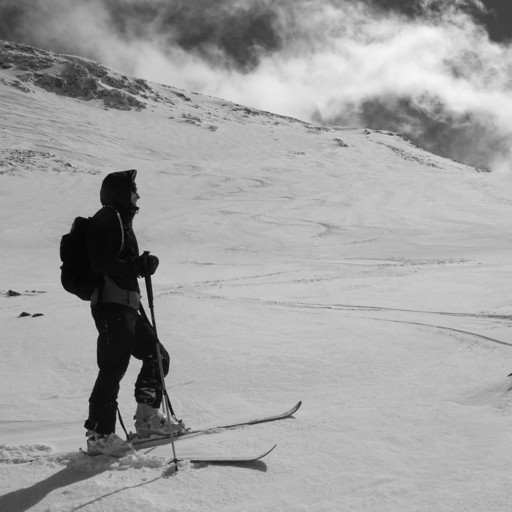
\includegraphics[width=.7\linewidth]{./out/orig-08}}
			\caption{Image originale}\label{Fig:orig-08}
		\end{minipage}\hfill
		\begin{minipage}{0.48\textwidth}
			\centering
			\fbox{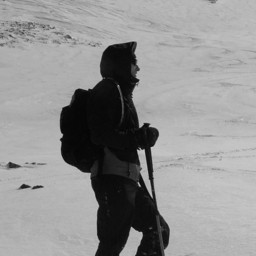
\includegraphics[width=.7\linewidth]{./out/resize-08}}
			\caption{Image redimensionnée}\label{Fig:resize-08}
		\end{minipage}
	\end{figure}

	\subsection{Seuillage de l'image}\label{subsec:1.2}

	On commence par modifier le programme \texttt{test\_grey.cpp} pour que les objets soient noirs et le fond blanc.
	On peut ensuite tester le seuillage de l'image avec différents seuils.
	Le plus pertinent semble être un seuil de 80, cela donne alors :
	% insert image and modified image
	\begin{figure}[!htb]
		\begin{minipage}{0.48\textwidth}
			\centering
			\fbox{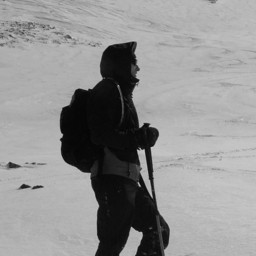
\includegraphics[width=.7\linewidth]{./out/resize-08}}
			\caption{Image redimensionnée}\label{Fig:resize-08-2}
		\end{minipage}\hfill
		\begin{minipage}{0.48\textwidth}
			\centering
			\fbox{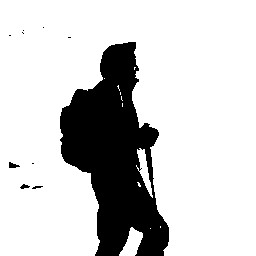
\includegraphics[width=.7\linewidth]{./out/test-grey-resize-08}}
			\caption{Image modifiée avec un seuil de 80}\label{Fig:test-grey-08}
		\end{minipage}
	\end{figure}

	\newpage
	\subsection{Erosion de l'image binaire}\label{subsec:1.3}

	On commence par créer un programme \texttt{erosion.cpp} pour effectuer l'érosion de l'image.
	Cela consiste à parcourir l'image et à remplacer chaque pixel par le maximum des pixels voisins.

	L'essentiel du code est le suivant : % insertion en image du code
	\begin{figure}[!htb]
		\centering
		\fbox{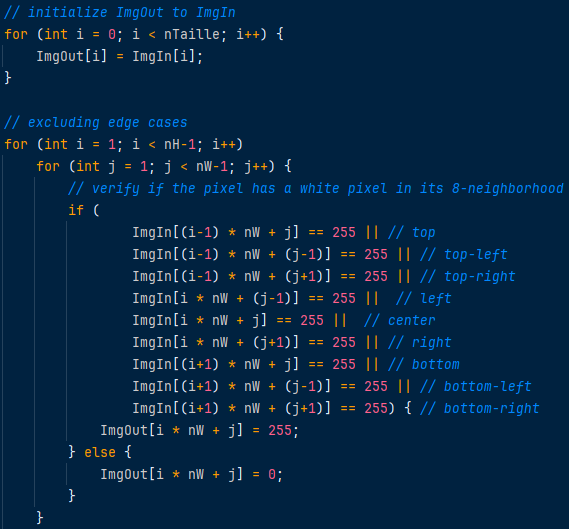
\includegraphics[width=.7\linewidth]{./out/erosion-code}}
		\caption{Code de l'érosion}\label{fig:erosion-code}
	\end{figure}

	On peut ensuite tester l'érosion de l'image avec l'image seuillée précédemment.
	Cela donne alors :
	% insert image and modified image
	\begin{figure}[!htb]
		\begin{minipage}{0.48\textwidth}
			\centering
			\fbox{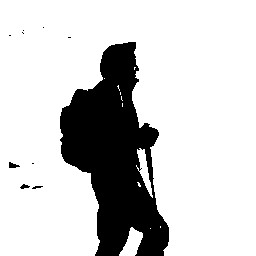
\includegraphics[width=.7\linewidth]{./out/test-grey-resize-08}}
			\caption{Image modifiée avec un seuil de 80}\label{Fig:test-grey-08-2}
		\end{minipage}\hfill
		\begin{minipage}{0.48\textwidth}
			\centering
			\fbox{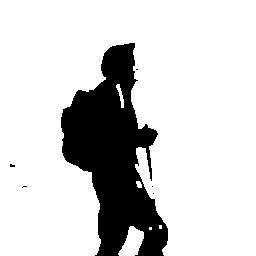
\includegraphics[width=.7\linewidth]{./out/erosion-resize-08}}
			\caption{Image modifiée avec l'érosion}\label{Fig:erosion-test-grey-08}
		\end{minipage}
	\end{figure}

	\newpage
	\section{Seuillage d'une image et dilatation de l'image binaire}\label{sec:2}

	\subsection{Dilatation de l'image binaire}\label{subsec:2.1}

	On commence par créer un programme \texttt{dilatation.cpp} pour effectuer la dilatation de l'image.
	Cela consiste à parcourir l'image et à remplacer chaque pixel par le minimum des pixels voisins.

	L'essentiel du code est le suivant : % insertion en image du code
	\begin{figure}[!htb]
		\centering
		\fbox{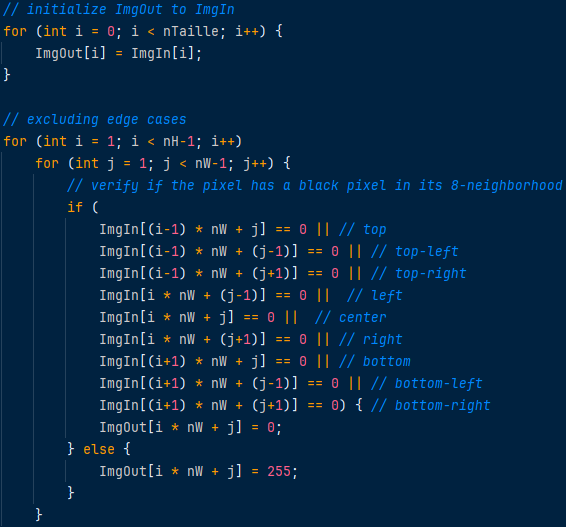
\includegraphics[width=.7\linewidth]{./out/dilatation-code}}
		\caption{Code de la dilatation}\label{fig:dilatation-code}
	\end{figure}

	On peut ensuite tester la dilatation de l'image avec l'image seuillée précédemment.
	Cela donne alors :
	% insert image and modified image
	\begin{figure}[!htb]
		\begin{minipage}{0.48\textwidth}
			\centering
			\fbox{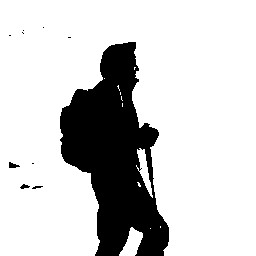
\includegraphics[width=.7\linewidth]{./out/test-grey-resize-08}}
			\caption{Image modifiée avec un seuil de 80}\label{Fig:test-grey-08-3}
		\end{minipage}\hfill
		\begin{minipage}{0.48\textwidth}
			\centering
			\fbox{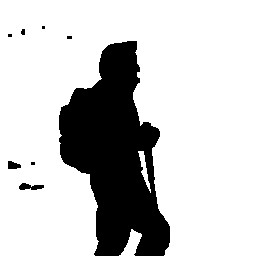
\includegraphics[width=.7\linewidth]{./out/dilatation-resize-08}}
			\caption{Image modifiée avec la dilatation}\label{Fig:dilatation-test-grey-08}
		\end{minipage}
	\end{figure}

	\newpage
	\section{Fermeture et ouverture d'une image et de l'image binaire}\label{sec:3}

	\subsection{Fermeture de l'image binaire}\label{subsec:3.1}

	On commence par créer un programme \texttt{fermeture.cpp} pour effectuer la fermeture de l'image.
	Cela consiste à effectuer une dilatation de l'image puis une érosion de l'image.
	Cela permet de fermer les trous dans les objets de l'image.

	L'essentiel du code est le suivant : % insertion en image du code
	\begin{figure}[!htb]
		\centering
		\fbox{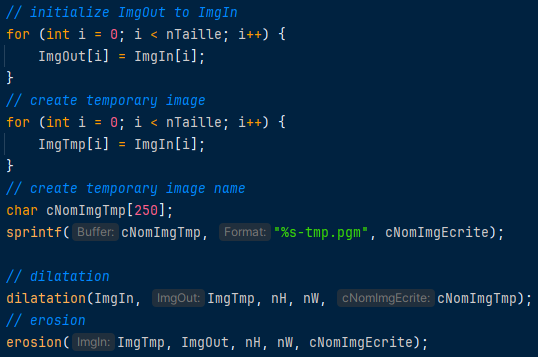
\includegraphics[width=.7\linewidth]{./out/fermeture-code}}
		\caption{Code de la fermeture}\label{fig:fermeture-code}
	\end{figure}

	L'essentiel du travail est de modifier les programmes précédents pour qu'ils puissent être utilisés dans ce
	programme.
	Pour cela, on crée des nouveaux fichiers sans \emph{main()} et extrait le contenu d'\texttt{image\_ppm.h} dans un
	fichier \emph{cpp}.

	On peut ensuite tester la fermeture de l'image avec l'image seuillée précédemment.
	Cela donne alors :
	% insert image and modified image
	\begin{figure}[!htb]
		\begin{minipage}{0.48\textwidth}
			\centering
			\fbox{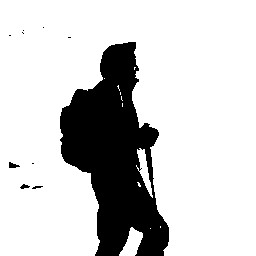
\includegraphics[width=.7\linewidth]{./out/test-grey-resize-08}}
			\caption{Image modifiée avec un seuil de 80}\label{Fig:test-grey-08-4}
		\end{minipage}\hfill
		\begin{minipage}{0.48\textwidth}
			\centering
			\fbox{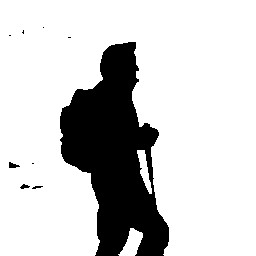
\includegraphics[width=.7\linewidth]{./out/fermeture-resize-08}}
			\caption{Image modifiée avec la fermeture}\label{Fig:fermeture-test-grey-08}
		\end{minipage}
	\end{figure}

	\newpage
	\subsection{Ouverture de l'image binaire}\label{subsec:3.2}

	On commence par créer un programme \texttt{ouverture.cpp} pour effectuer l'ouverture de l'image.
	Cela consiste à effectuer une érosion de l'image puis une dilatation de l'image.
	Cela permet de supprimer les petits objets de l'image.

	L'essentiel du code est le suivant : % insertion en image du code
	\begin{figure}[!htb]
		\centering
		\fbox{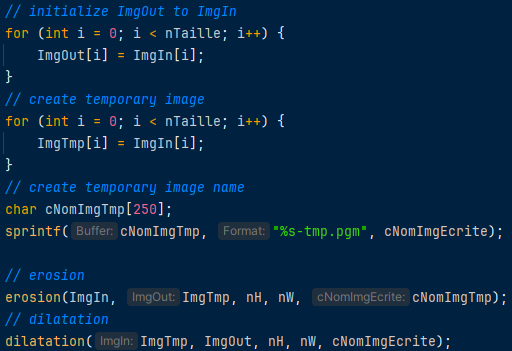
\includegraphics[width=.7\linewidth]{./out/ouverture-code}}
		\caption{Code de l'ouverture}\label{Fig:ouverture-code}
	\end{figure}

	On peut ensuite tester l'ouverture de l'image avec l'image seuillée précédemment.
	Cela donne alors :
	% insert image and modified image
	\begin{figure}[!htb]
		\begin{minipage}{0.48\textwidth}
			\centering
			\fbox{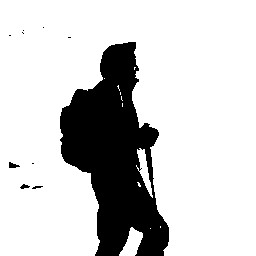
\includegraphics[width=.7\linewidth]{./out/test-grey-resize-08}}
			\caption{Image modifiée avec un seuil de 80}\label{Fig:test-grey-08-5}
		\end{minipage}\hfill
		\begin{minipage}{0.48\textwidth}
			\centering
			\fbox{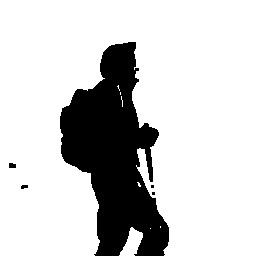
\includegraphics[width=.7\linewidth]{./out/ouverture-resize-08}}
			\caption{Image modifiée avec l'ouverture}\label{Fig:ouverture-test-grey-08}
		\end{minipage}
	\end{figure}

	\newpage
	\subsection{Enchainement de fermeture et ouverture}\label{subsec:3.3}

	On peut ensuite enchaîner la fermeture et l'ouverture de l'image pour obtenir une image plus propre.
	Cela donne alors :
	% insert original then closed then reopened image
	\begin{figure}[!htb]
		\begin{minipage}{0.30\textwidth}
			\centering
			\fbox{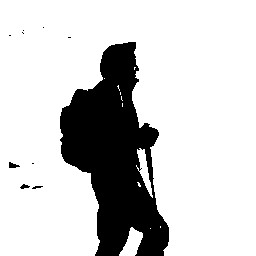
\includegraphics[width=.7\linewidth]{./out/test-grey-resize-08}}
			\caption{Image modifiée avec un seuil de 80}\label{Fig:test-grey-08-6}
		\end{minipage}\hfill
		\begin{minipage}{0.30\textwidth}
			\centering
			\fbox{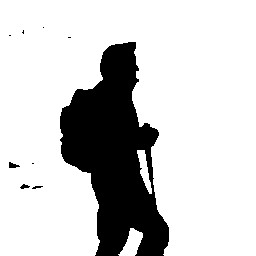
\includegraphics[width=.7\linewidth]{./out/fermeture-resize-08}}
			\caption{Image modifiée avec fermeture}\label{Fig:fermeture-ouverture-test-grey-08}
		\end{minipage}\hfill
		\begin{minipage}{0.30\textwidth}
			\centering
			\fbox{
\includegraphics[width=.7\linewidth]{./out/ouverture-fermeture-resize-08}}
			\caption{Image modifiée avec fermeture puis ouverture}\label{Fig:ouverture-fermeture-test-grey-08}
		\end{minipage}
	\end{figure}

	\subsection{Impact cumulatif de la fermeture et de l'ouverture}\label{subsec:3.4}

	On peut ensuite tester l'impact cumulatif de la fermeture et de l'ouverture de l'image.
	On procède d'abord à 3 dilatations, 6 érosions et enfin 3 dilatations.

	Cela donne alors :
	% insert original then modified image
	\begin{figure}[!htb]
		\begin{minipage}{0.48\textwidth}
			\centering
			\fbox{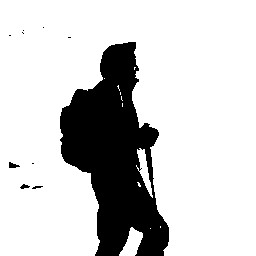
\includegraphics[width=.7\linewidth]{./out/test-grey-resize-08}}
			\caption{Image modifiée avec un seuil de 80}\label{Fig:test-grey-08-7}
		\end{minipage}\hfill
		\begin{minipage}{0.48\textwidth}
			\centering
			\fbox{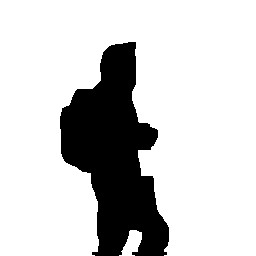
\includegraphics[width=.7\linewidth]{./out/edil3-resize-08}}
			\caption{Image modifiée avec cumul}\label{Fig:fermeture-ouverture-test-grey-08-2}
		\end{minipage}
	\end{figure}

	\newpage
	\section{Segmentation d'une image}\label{sec:4}

	\subsection{Detection de contours}\label{subsec:4.1}

	On commence par créer un programme \texttt{difference.cpp} pour effectuer la détection de contours de l'image.
	Cela consiste à effectuer une dilatation de l'image puis d'observer la différence entre l'image dilatée et l'image
	originale.

	L'essentiel du code est le suivant : % insertion en image du code
	\begin{figure}[!htb]
		\centering
		\fbox{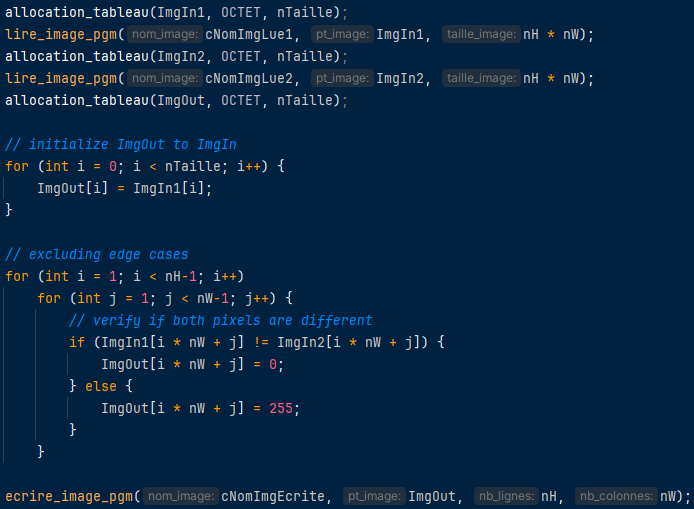
\includegraphics[width=.7\linewidth]{./out/difference-code}}
		\caption{Code de la détection de contours}\label{Fig:difference-code}
	\end{figure}

	On peut ensuite tester la détection de contours de l'image avec l'image seuillée précédemment.
	Cela donne alors :
	% insert original then modified image
	\begin{figure}[!htb]
		\begin{minipage}{0.48\textwidth}
			\centering
			\fbox{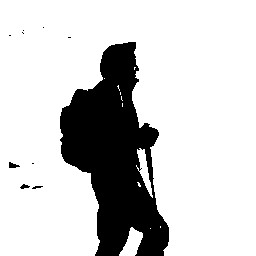
\includegraphics[width=.7\linewidth]{./out/test-grey-resize-08}}
			\caption{Image modifiée avec un seuil de 80}\label{Fig:test-grey-08-8}
		\end{minipage}\hfill
		\begin{minipage}{0.48\textwidth}
			\centering
			\fbox{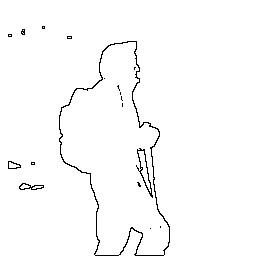
\includegraphics[width=.7\linewidth]{./out/difference-tg-dil-resize-08}}
			\caption{Image modifiée avec la détection de contours}\label{Fig:difference-test-grey-08}
		\end{minipage}
	\end{figure}

	\newpage
	\section{Bonus : extension aux images en niveaux de gris}\label{sec:5}

	\subsection{Erosion de l'image en niveaux de gris}\label{subsec:5.1}

	On commence par créer un programme \texttt{erosion\_grey.cpp} pour effectuer l'érosion de l'image en niveaux de
	gris.
	Cela consiste à parcourir l'image et à remplacer chaque pixel par le maximum des pixels voisins.

	L'essentiel du code est le suivant : % insertion en image du code
	\begin{figure}[!htb]
		\centering
		\fbox{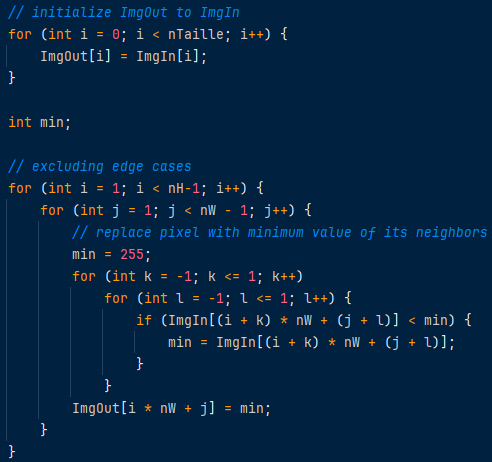
\includegraphics[height=.6\linewidth]{./out/erosion-grey-code}}
		\caption{Code de l'érosion en niveaux de gris}\label{Fig:erosion-grey-code}
	\end{figure}

	On peut ensuite tester l'érosion de l'image avec l'image en niveaux de gris \texttt{08.pgm}.
	Cela donne alors :
	% insert original then modified image
	\begin{figure}[!htb]
		\begin{minipage}{0.48\textwidth}
			\centering
			\fbox{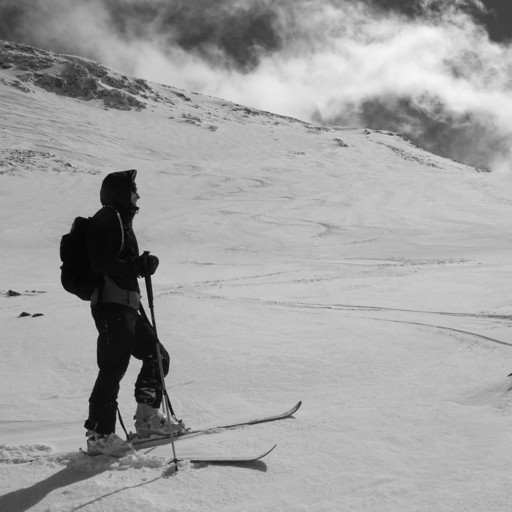
\includegraphics[width=.7\linewidth]{./out/orig-08}}
			\caption{Image originale}\label{Fig:orig-08-2}
		\end{minipage}\hfill
		\begin{minipage}{0.48\textwidth}
			\centering
			\fbox{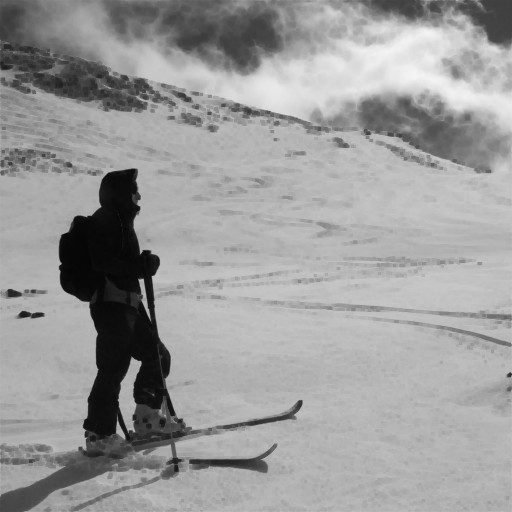
\includegraphics[width=.7\linewidth]{./out/erosion-grey-08}}
			\caption{Image modifiée avec l'érosion en niveaux de gris}\label{Fig:erosion-grey-08}
		\end{minipage}
	\end{figure}

	\newpage
	\subsection{Dilatation de l'image en niveaux de gris}\label{subsec:5.2}

	On commence par créer un programme \texttt{dilatation\_grey.cpp} pour effectuer la dilatation de l'image en niveaux
	de gris.
	Cela consiste à parcourir l'image et à remplacer chaque pixel par le minimum des pixels voisins.

	L'essentiel du code est le suivant : % insertion en image du code
	\begin{figure}[!htb]
		\centering
		\fbox{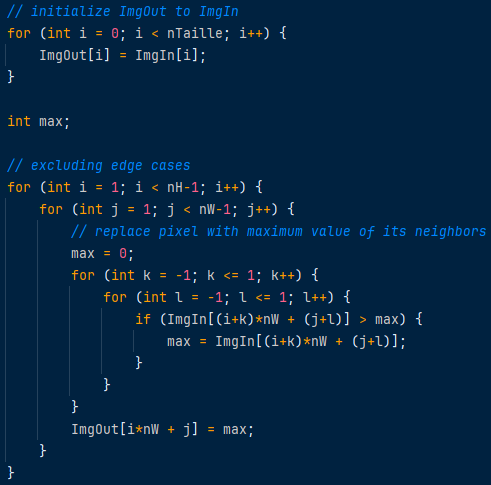
\includegraphics[width=.7\linewidth]{./out/dilatation-grey-code}}
		\caption{Code de la dilatation en niveaux de gris}\label{Fig:dilatation-grey-code}
	\end{figure}

	On peut ensuite tester la dilatation de l'image avec l'image en niveaux de gris \texttt{08.pgm}.
	Cela donne alors :
	% insert original then modified image
	\begin{figure}[!htb]
		\begin{minipage}{0.48\textwidth}
			\centering
			\fbox{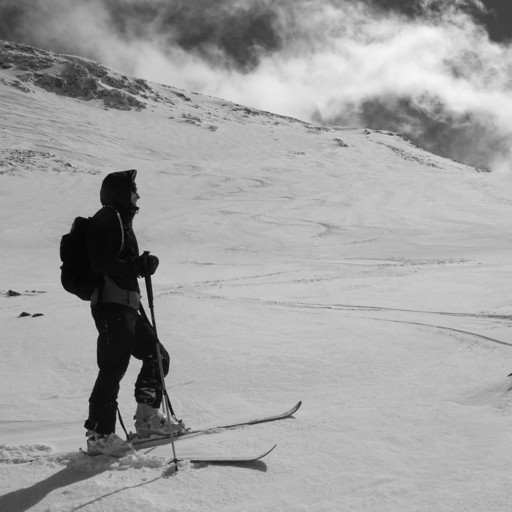
\includegraphics[width=.7\linewidth]{./out/orig-08}}
			\caption{Image originale}\label{Fig:orig-08-3}
		\end{minipage}\hfill
		\begin{minipage}{0.48\textwidth}
			\centering
			\fbox{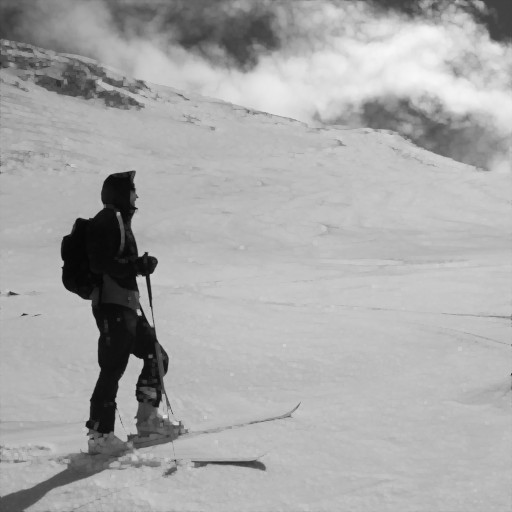
\includegraphics[width=.7\linewidth]{./out/dilatation-grey-08}}
			\caption{Image modifiée avec la dilatation en niveaux de gris}\label{Fig:dilatation-grey-08}
		\end{minipage}
	\end{figure}

	\newpage
	\subsection{Fermeture de l'image en niveaux de gris}\label{subsec:5.3}

	On commence par créer un programme \texttt{fermeture\_grey.cpp} pour effectuer la fermeture de l'image en niveaux
	de gris.
	Cela consiste à effectuer une dilatation de l'image puis une érosion de l'image.
	Cela permet de fermer les trous dans les objets de l'image.

	L'essentiel du code est le suivant : % insertion en image du code
	\begin{figure}[!htb]
		\centering
		\fbox{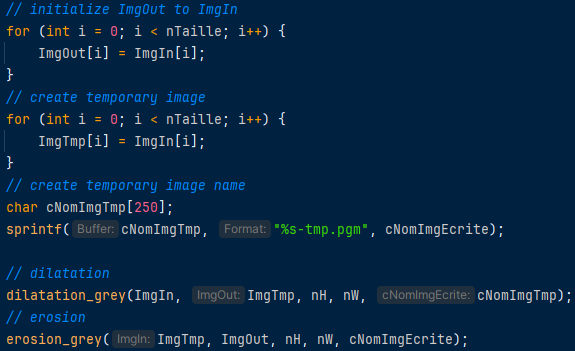
\includegraphics[width=.7\linewidth]{./out/fermeture-grey-code}}
		\caption{Code de la fermeture en niveaux de gris}\label{Fig:fermeture-grey-code}
	\end{figure}

	On peut ensuite tester la fermeture de l'image avec l'image en niveaux de gris \texttt{08.pgm}.
	Cela donne alors :
	% insert original then modified image
	\begin{figure}[!htb]
		\begin{minipage}{0.48\textwidth}
			\centering
			\fbox{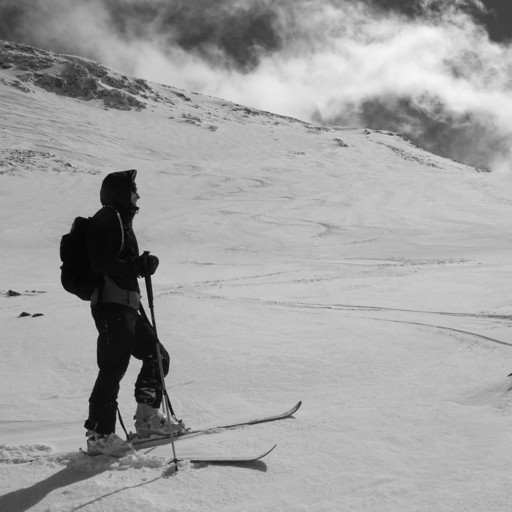
\includegraphics[width=.7\linewidth]{./out/orig-08}}
			\caption{Image originale}\label{Fig:orig-08-4}
		\end{minipage}\hfill
		\begin{minipage}{0.48\textwidth}
			\centering
			\fbox{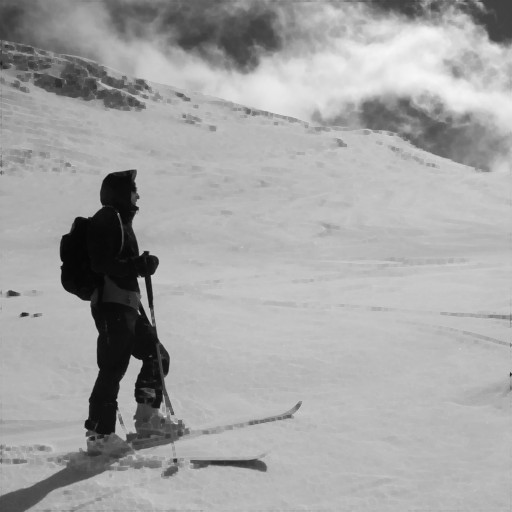
\includegraphics[width=.7\linewidth]{./out/fermeture-grey-08}}
			\caption{Image modifiée avec la fermeture en niveaux de gris}\label{Fig:fermeture-grey-08}
		\end{minipage}
	\end{figure}

	\newpage
	\subsection{Ouverture de l'image en niveaux de gris}\label{subsec:5.4}

	On commence par créer un programme \texttt{ouverture\_grey.cpp} pour effectuer l'ouverture de l'image en niveaux
	de gris.
	Cela consiste à effectuer une érosion de l'image puis une dilatation de l'image.
	Cela permet de supprimer les petits objets de l'image.

	L'essentiel du code est le suivant : % insertion en image du code
	\begin{figure}[!htb]
		\centering
		\fbox{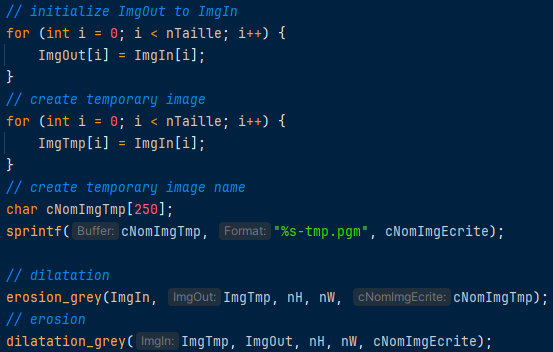
\includegraphics[width=.7\linewidth]{./out/ouverture-grey-code}}
		\caption{Code de l'ouverture en niveaux de gris}\label{Fig:ouverture-grey-code}
	\end{figure}

	On peut ensuite tester l'ouverture de l'image avec l'image en niveaux de gris \texttt{08.pgm}.
	Cela donne alors :
	% insert original then modified image
	\begin{figure}[!htb]
		\begin{minipage}{0.48\textwidth}
			\centering
			\fbox{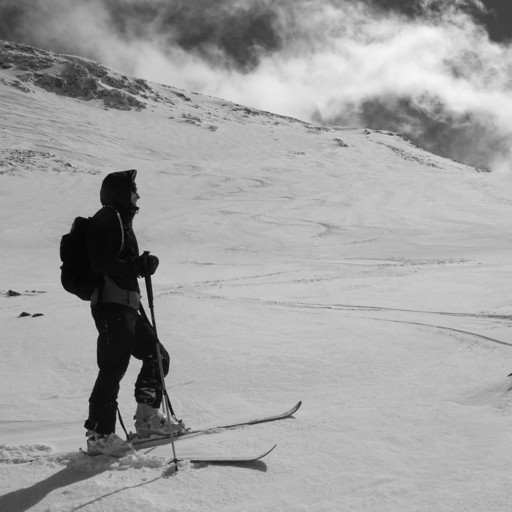
\includegraphics[width=.7\linewidth]{./out/orig-08}}
			\caption{Image originale}\label{Fig:orig-08-5}
		\end{minipage}\hfill
		\begin{minipage}{0.48\textwidth}
			\centering
			\fbox{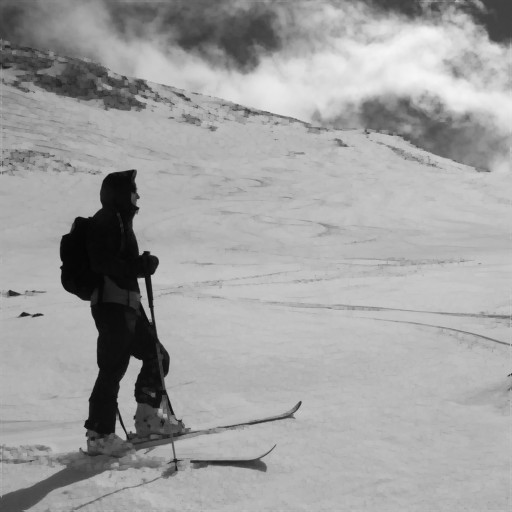
\includegraphics[width=.7\linewidth]{./out/ouverture-grey-08}}
			\caption{Image modifiée avec l'ouverture en niveaux de gris}\label{Fig:ouverture-grey-08}
		\end{minipage}
	\end{figure}

	\subsection{Enchainement de fermeture et ouverture en niveaux de gris}\label{subsec:5.5}

	On peut ensuite enchaîner la fermeture et l'ouverture de l'image pour obtenir une image plus propre.
	Cela donne alors :
	% insert original then closed then reopened image
	\begin{figure}[!htb]
		\begin{minipage}{0.30\textwidth}
			\centering
			\fbox{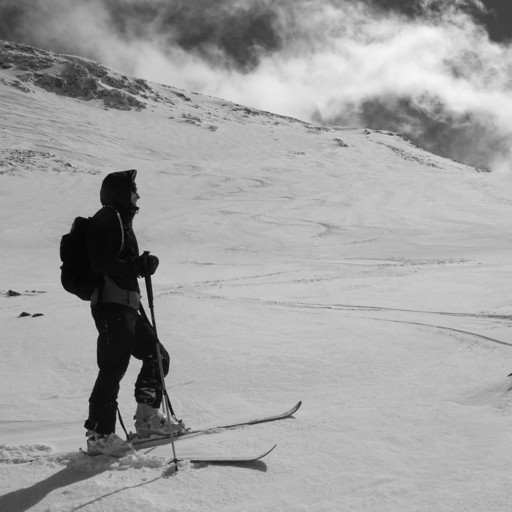
\includegraphics[width=.7\linewidth]{./out/orig-08}}
			\caption{Image originale}\label{Fig:orig-08-6}
		\end{minipage}\hfill
		\begin{minipage}{0.30\textwidth}
			\centering
			\fbox{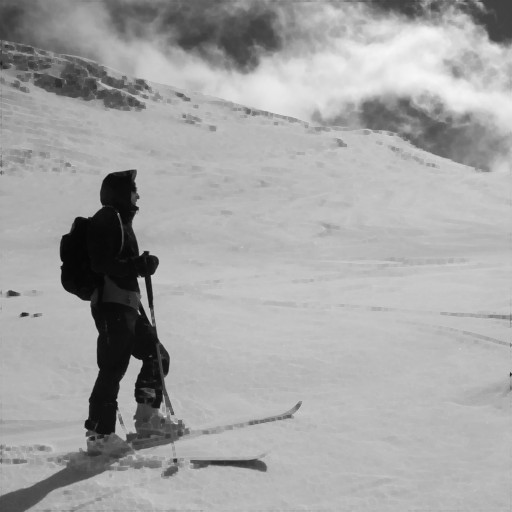
\includegraphics[width=.7\linewidth]{./out/fermeture-grey-08}}
			\caption{Image modifiée avec fermeture}\label{Fig:fermeture-ouverture-grey-08}
		\end{minipage}\hfill
		\begin{minipage}{0.30\textwidth}
			\centering
			\fbox{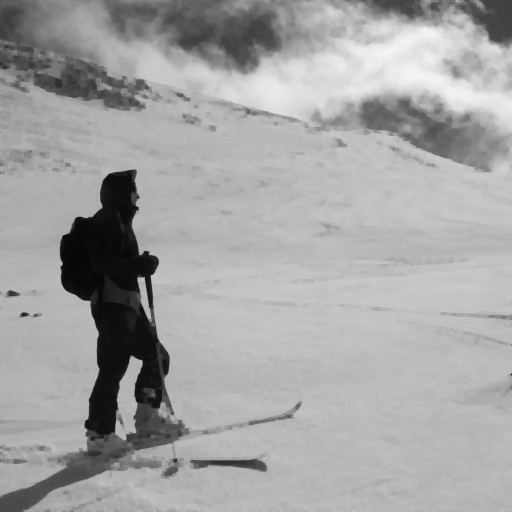
\includegraphics[width=.7\linewidth]{./out/ouverture-fermeture-grey-08}}
			\caption{Image modifiée avec fermeture puis ouverture}\label{Fig:ouverture-fermeture-grey-08}
		\end{minipage}
	\end{figure}

	\newpage
	\subsection{Impact cumulatif de la fermeture et de l'ouverture en niveaux de gris}\label{subsec:5.6}

	On peut ensuite tester l'impact cumulatif de la fermeture et de l'ouverture de l'image en niveaux de gris.
	On procède d'abord à 3 dilatations, 6 érosions et enfin 3 dilatations.

	Cela donne alors :
	% insert original then modified image
	\begin{figure}[!htb]
		\begin{minipage}{0.48\textwidth}
			\centering
			\fbox{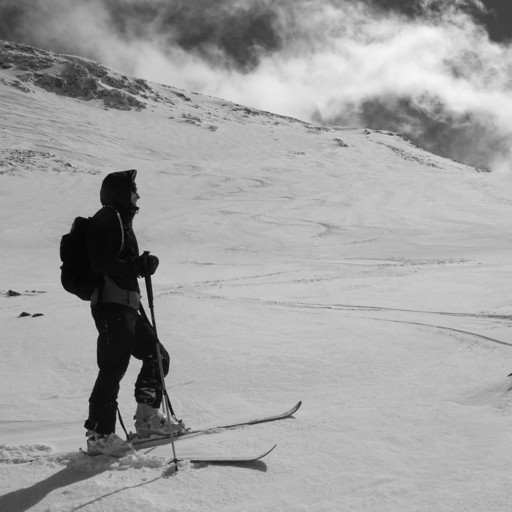
\includegraphics[width=.7\linewidth]{./out/orig-08}}
			\caption{Image originale}\label{Fig:orig-08-7}
		\end{minipage}\hfill
		\begin{minipage}{0.48\textwidth}
			\centering
			\fbox{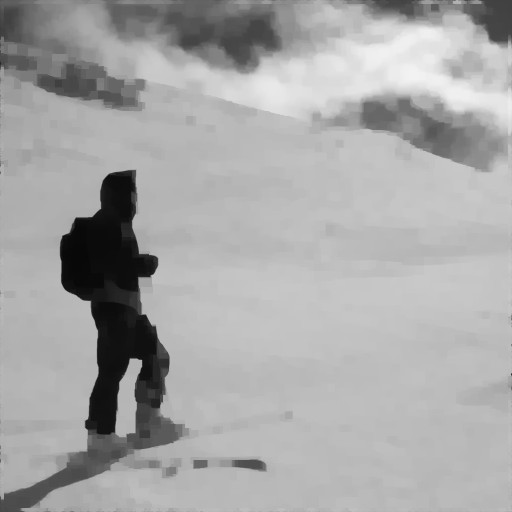
\includegraphics[width=.7\linewidth]{./out/edil3-erod6-08}}
			\caption{Image modifiée avec cumul}\label{Fig:fermeture-ouverture-grey-08-2}
		\end{minipage}
	\end{figure}


	\newpage
	\subsection{Segmentation d'une image en niveaux de gris}\label{subsec:5.7}

	On peut directement réutiliser le programme \texttt{difference.cpp} pour effectuer la segmentation de l'image en
	niveaux de gris.

	On peut ensuite tester la segmentation de l'image avec l'image en niveaux de gris \texttt{08.pgm}.
	Cela donne alors :
	% insert original then modified image
	\begin{figure}[!htb]
		\begin{minipage}{0.48\textwidth}
			\centering
			\fbox{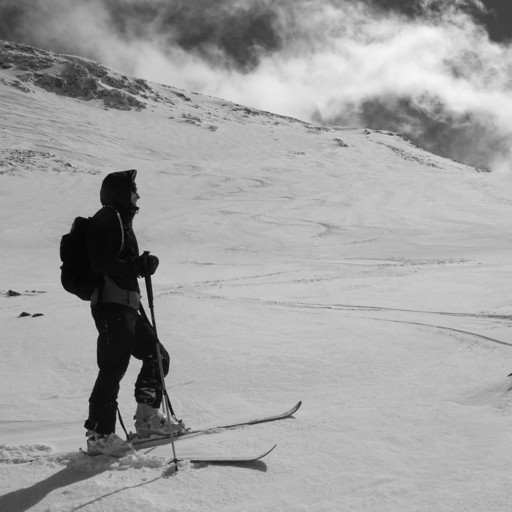
\includegraphics[width=.5\linewidth]{./out/orig-08}}
			\caption{Image originale}\label{Fig:orig-08-8}
		\end{minipage}\hfill
		\begin{minipage}{0.48\textwidth}
			\centering
			\fbox{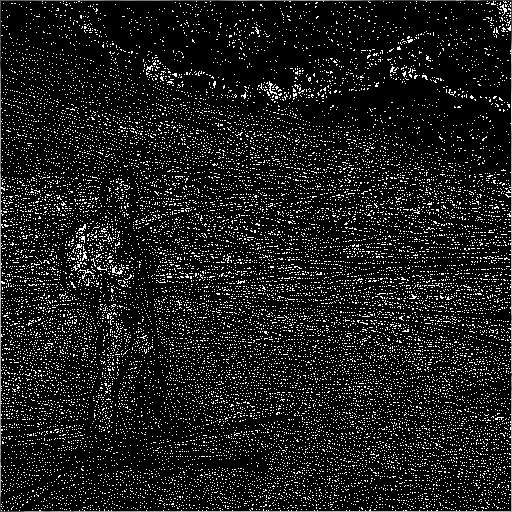
\includegraphics[width=.5\linewidth]{./out/difference-grey-08}}
			\caption{Image modifiée avec la difference en niveaux de gris}\label{Fig:segmentation-grey-08}
		\end{minipage}
	\end{figure}

	On constate que cela donne un résultat très surprenant, on peut alors essayer d'adapter le programme pour qu'il
	soit plus pertinent.
	On décide donc de regarder si la différence entre deux pixels est supérieure à un certain seuil.
	Le programme \texttt{difference\_grey\_seuil.cpp} est ainsi créé pour un meilleur résultat.

	Le code est le suivant : % insertion en image du code
	\begin{figure}[!htb]
		\centering
		\fbox{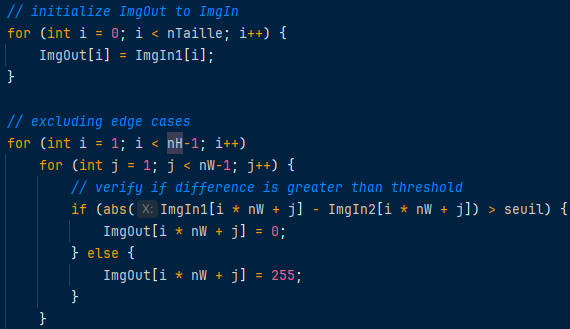
\includegraphics[width=.5\linewidth]{./out/difference-grey-seuil-code}}
		\caption{Code de la différence en niveaux de gris avec seuil}\label{Fig:difference-grey-seuil-code}
	\end{figure}

	On peut ensuite tester la segmentation de l'image avec l'image en niveaux de gris \texttt{08.pgm}.
	Pour des différents seuils, on obtient les transformations suivantes :
	% insert original and 3 modified images
	\begin{figure}[!htb]
		\begin{minipage}{0.22\textwidth}
			\centering
			\fbox{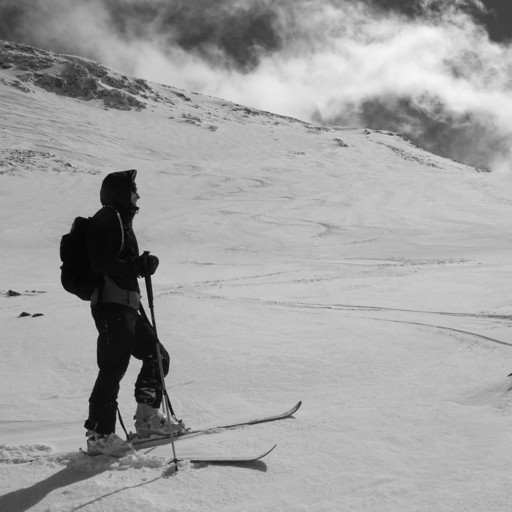
\includegraphics[width=.8\linewidth]{./out/orig-08}}
			\caption{Image originale}\label{Fig:orig-08-9}
		\end{minipage}\hfill
		\begin{minipage}{0.22\textwidth}
			\centering
			\fbox{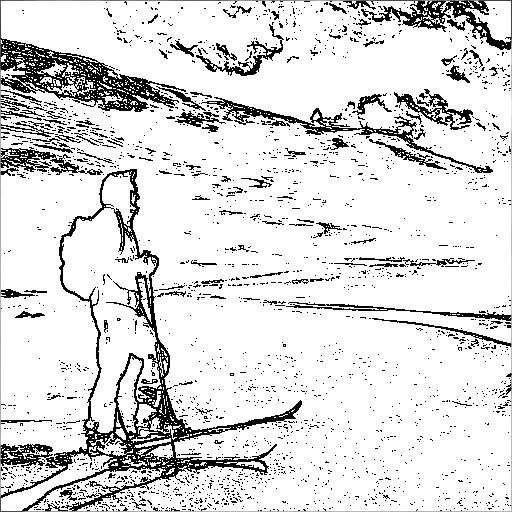
\includegraphics[width=.8\linewidth]{./out/difference-grey-08-10}}
			\caption{Image modifiée avec seuil de 10}\label{Fig:segmentation-grey-08-10}
		\end{minipage}\hfill
		\begin{minipage}{0.22\textwidth}
			\centering
			\fbox{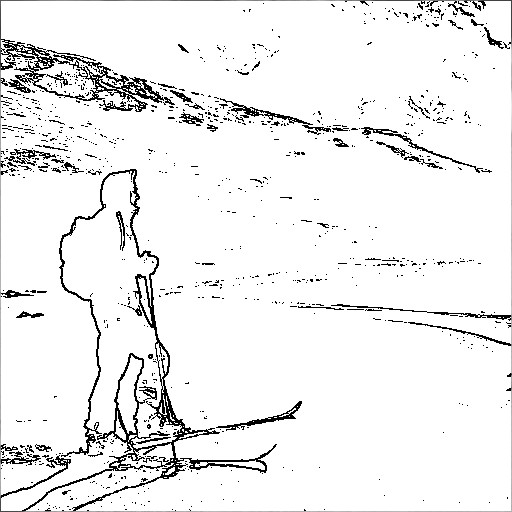
\includegraphics[width=.8\linewidth]{./out/difference-grey-08-20}}
			\caption{Image modifiée avec seuil de 20}\label{Fig:segmentation-grey-08-20}
		\end{minipage}\hfill
		\begin{minipage}{0.22\textwidth}
			\centering
			\fbox{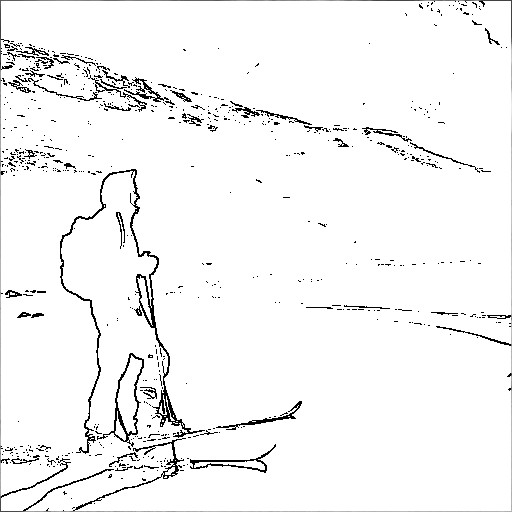
\includegraphics[width=.8\linewidth]{./out/difference-grey-08-30}}
			\caption{Image modifiée avec seuil de 30}\label{Fig:segmentation-grey-08-30}
		\end{minipage}\hfill
	\end{figure}

	\newpage
	\section{Conclusion}\label{sec:6}

	En conclusion, on a pu voir que les opérations morphologiques permettent de modifier les images de manière
	intéressante.
	On a pu voir que l'érosion et la dilatation permettent de modifier les images binaires, la fermeture et
	l'ouverture permettent de nettoyer les images binaires et la détection de contours permet de segmenter les images
	en niveaux de gris.
	On a pu voir que l'extension aux images en niveaux de gris est possible et permet de segmenter les images de manière
	intéressante.


\end{document}

